%% This is an example first chapter.  You should put chapter/appendix that you
%% write into a separate file, and add a line \include{yourfilename} to
%% main.tex, where `yourfilename.tex' is the name of the chapter/appendix file.
%% You can process specific files by typing their names in at the 
%% \files=
%% prompt when you run the file main.tex through LaTeX.
\chapter{Application of Best-Response Tensor-Train-Decomposition-Based Value Iteration}\label{chp:examples}
In this chapter, we apply the BR-TT-VI algorithm to two problem instances. The first problem, a four-dimensional pursuit-evasion game will be solved with both a traditional value iteration algorithm (VI), \Cref{DPBRalg}, and the BR-TT-VI algorithm, \Cref{BRTVIalg}. This will allow for comparisons between the two algorithms to demonstrate the benefits of using BR-TT-VI. Next, a six-dimensional pursuit-evasion problem will be solved that demonstrates BR-TT-VI's ability to efficiently compute a solution for a problem that would take VI days if not weeks to solve. In total, this chapter will demonstrate the contributions that the BR-TT-VI algorithm provides to solving pursuit-evasion games.  

\section{Four-Dimensional Problem}
The four-dimensional pursuit-evasion problem used here is simple enough to be solved analytically, with VI, and with BR-TT-VI. This problem is used as a benchmark to show the accuracy of the BR-TT-VI approximation and demonstrate the advantages of using BR-TT-VI over VI. This section will start with a definition of the four-dimensional pursuit-evasion problem as well as a brief explanation of the optimal analytic solution to the problem. Next, it will be explained how both VI and BR-TT-VI were accomplished and the results of these algorithms. Finally, a comparison will be made between the results of VI and BR-TT-VI.   
\subsection{Problem Definition}
The four-dimensional pursuit-evasion problem used here has the pursuer attempting to reduce the distance to or capture the evader, while the evader attempts to maximize the distance between itself and the pursuer. To do this, a pursuer and an evader are modeled in a $10 \times 10$ two-dimensional field with simple Euclidean dynamics. This results in the four-dimensional state space where the states are the x position of the pursuer $x_1$, the y position of the pursuer $y_1$, the x position of the evader $x_2$, and the y position of the evader $y_2$. This results in a state space such that $z_i = (x_1,y_1,x_2,y_2)$. Each of the dimensions are bounded as follows:
\begin{eqnarray*}
x_1 & \in & [0,10]\\
y_1 & \in & [0,10]\\
x_2 & \in & [0,10]\\
y_2 & \in & [0,10].
\end{eqnarray*} 
Both the pursuer and the evader have two controls for their $x$ and $y$ velocity respectively, $u_1 = (Vx_1,Vy_1)$ and $u_2 = (Vx_2,Vy_2)$. These velocities are also bounded:
\begin{eqnarray*}
Vx_1 & \in & [-1,1]\\
Vy_1 & \in & [-1,1]\\
Vx_2 & \in & [-0.5,0.5]\\
Vy_2 & \in & [-0.5,0.5].
\end{eqnarray*} 
Furthermore, the following system dynamics are used:
\begin{eqnarray}
x_1^{k+1} & = & x_1^k +Vx_1dt,\label{eqns1.1} \\
y_1^{k+1} & = & y_1^k +Vy_1dt,\label{eqns1.2}\\
x_2^{k+1} & = & x_2^k +Vx_2dt,\label{eqns1.3}\\
y^{k+1}_2 & = & y_2^k +Vy_2dt.\label{eqns1.4}
\end{eqnarray}
Each dimension is discretized into 21 equally spaced states for a total of $21^4 \approx 2\cdot10^5$ discrete states. This discretization was chosen as it creates a state for every $0.5$ units:
\begin{eqnarray*}
x_1 & \in & \left\{0,0.5,1,1.5,2,2.5,3,3.5,4,4.5,5,5.5,6,6.5,7,7.5,8,8.5,9,9.5,10\right\}\\
y_1 & \in & \left\{0,0.5,1,1.5,2,2.5,3,3.5,4,4.5,5,5.5,6,6.5,7,7.5,8,8.5,9,9.5,10\right\}\\
x_2 & \in & \left\{0,0.5,1,1.5,2,2.5,3,3.5,4,4.5,5,5.5,6,6.5,7,7.5,8,8.5,9,9.5,10\right\}\\
y_2 & \in & \left\{0,0.5,1,1.5,2,2.5,3,3.5,4,4.5,5,5.5,6,6.5,7,7.5,8,8.5,9,9.5,10\right\}.
\end{eqnarray*} 
 
Value iteration can be used to solve for the optimal cost at each state. The problem is modeled as in \Cref{peprobdes}. A state cost function based on the distance between the pursuer and evader was chosen: 
\begin{equation}\label{4cost}
G(z_i,u_1,u_2)= 10+(x_1-x_2)^2+(y_1-y_2)^2.
\end{equation}
The constant of $10$ is added to provided a buffer for the BR-TT-VI approximation in order to prevent negative values. A discount factor of $\gamma = 0.7$ was chosen because it provided just enough look-ahead to predict the opponent's next state without allowing predictions of moves made multiple seconds later to influence the state cost. Applying the state cost function and discount factor to \Cref{pbell} results in the update functions for the four-dimensional pursuit-evasion problem:
\begin{equation}\label{4pbell}
J_p^{(k+1,K)}(z_i)= \underset{u_1 }{\operatorname{min }}[10+(x_1-x_2)^2+(y_1-y_2)^2+0.7 J_p^{(k,K)}(z_j|z_i,u_1,u_2^K)],
\end{equation}
\begin{equation}\label{4ebell}
J_e^{(k+1,K)}(z_i)= \underset{u_2 }{\operatorname{max }}[10+(x_1-x_2)^2+(y_1-y_2)^2+0.7 J_e^{(k,K)}(z_j|z_i,u_1^K,u_2)].
\end{equation} 
Running \Cref{DPBRalg} with \Cref{4pbell,4ebell} results in the given optimal value functions:
\begin{equation}\label{4pbropt}
J_p^{(*,*)}(z_i)= \underset{u_1 }{\operatorname{min }}[10+(x_1-x_2)^2+(y_1-y_2)^2+0.7 J_p^{(*,*)}(z_j|z_i,u_1,u_2^*)],
\end{equation}
\begin{equation}\label{4ebropt}
J_e^{(*,*)}(z_i)= \underset{u_2 }{\operatorname{max }}[10+(x_1-x_2)^2+(y_1-y_2)^2+0.7 J_e^{(*,*)}(z_j|z_i,u_1^*,u_2)].
\end{equation}    
These optimal value functions, \Cref{4pbropt,4ebropt}, can be used to solve the following pursuit-evasion optimization problem:
\begin{eqnarray}\label{4opt}
&&\underset{u_1 }{\operatorname{min \textnormal{ } }}\underset{u_2 }{\operatorname{max }}[\int_{0}^{T}e^{-0.7t}(10+(x_1(t)-x_2(t))^2+(y_1(t)-y_2(t))^2)dt]\\
&\textnormal{s.t.}&(\ref{eqns1.1}-\ref{eqns1.4}).
\end{eqnarray}

\subsection{Analytical Solution}
The four-dimensional problem has a simple analytic solution because the dimensions are separable. This problem has separable dimensions in that any change in one dimension does not affect a change in the other dimension. Furthermore, the controls are completely separate in regard to dimension. For example, choosing a certain control in the $x$ dimension does not prevent choosing a control in the $y$ dimension. Because of this the problem can be viewed as simultaneously solving two one-dimensional problems where the pursuer is trying to minimize $|x_1-x_2|$ and $|y_1-y_2|$ while the evader attempts to maximize these functions. For the pursuer, the optimal solution is:
\begin{equation}\label{puroptx}
Vx_1^*= \underset{Vx_1 }{\operatorname{arg min }}[((x_1 + Vx_1dt)-(x_2+Vx_2dt))^2],
\end{equation}
\begin{equation}\label{puropty}
Vy_1^*= \underset{Vy_1 }{\operatorname{arg min }}[((y_1 + Vy_1dt)-(y_2+Vy_2dt))^2].
\end{equation}
The optimal solution for the evader is then:
\begin{equation}\label{evadoptx}
Vx_2^*= \underset{Vx_2 }{\operatorname{arg max }}[((x_1 + Vx_1dt)-(x_2+Vx_2dt))^2],
\end{equation}
\begin{equation}\label{evadopty}
Vy_2^*= \underset{Vy_2 }{\operatorname{arg max }}[((y_1 + Vy_1dt)-(y_2+Vy_2dt))^2].
\end{equation}
These analytically solutions can be used to check the validity of the results of both VI and BR-TT-VI. 

\subsection{Traditional Value Iteration}
Before running the best response algorithm based on traditional value iteration (\Cref{DPBRalg}) both the pursuer and evader VI algorithms were run for 100 iterations to better characterize the algorithm when run past completion. First, both the pursuer and evader state cost were set to initialized such that $J^{(0,0)}_p(z_i) = (x_1-x_2)^2+(y_1-y_2)^2$ and $J^{(0,0)}_e(z_i) = (x_1-x_2)^2+(y_1-y_2)^2$. Next, the pursuer value iteration is run for one hundred iterations. It took approximately 90 minutes to run these one hundred iterations of pursuer value iteration, \Cref{4DVIrt}. The evolution of the pursuer state cost can be seen  in \Cref{100IR4DTPCP}. Take note of the minimal difference in the state cost between ten and a hundred iterations. Notice that the average norm converges to the optimal average norm, \Cref{100IR4DTnp}, and the difference between the average norm decreases exponentially fast, \Cref{100IR4DTdnp}. The breakdown of the decrease around the $95^{th}$ iteration is due to rounding error caused by the precision of float values.  
\begin{figure}[h!]
\centering
\begin{subfigure}[t]{0.475\textwidth}
	\centering
	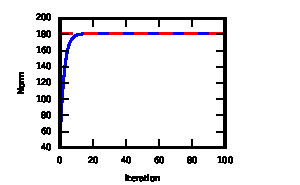
\includegraphics[width=\textwidth]{100IR4DTradPursnormplot}
	\caption{Average norm of the pursuer state cost with red dashed line as the average norm of the optimal value}
	\label{100IR4DTnp}
\end{subfigure}
\hfill
\begin{subfigure}[t]{0.475\textwidth}
	\centering
	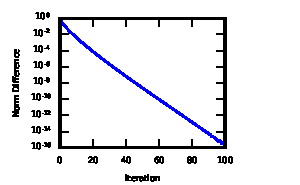
\includegraphics[width=\textwidth]{100IR4DTradPursdiffNormplot}
	\caption{Normalized difference in average norm between sequential pursuer state costs}
	\label{100IR4DTdnp}
\end{subfigure}
\caption{Diagnostic results of running 100 Iterations of Pursuit Value Iteration}
\label{100IR4DTdiag}
\end{figure} 
\begin{figure}
\centering
\begin{subfigure}[b]{0.475\textwidth}
	\centering
	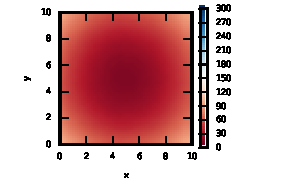
\includegraphics[width=\textwidth]{100IR4DTradPurspurscolorplot0}
	\caption{1 Iteration }
	\label{100IR4DTPCP0}
\end{subfigure}
\hfill
\begin{subfigure}[b]{0.475\textwidth}
	\centering
	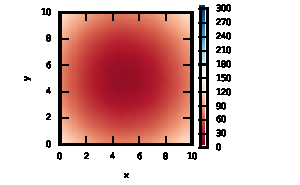
\includegraphics[width=\textwidth]{100IR4DTradPurspurscolorplot1}
	\caption{2 Iterations}
	\label{100IR4DTPCP1}
\end{subfigure}
\vskip\baselineskip
\begin{subfigure}[b]{0.475\textwidth}
	\centering
	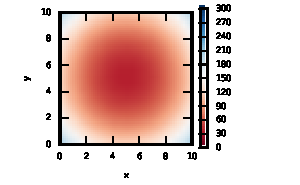
\includegraphics[width=\textwidth]{100IR4DTradPurspurscolorplot9}
	\caption{10 Iterations}
	\label{100IR4DTPCP9}
\end{subfigure}
\quad
\begin{subfigure}[b]{0.475\textwidth}
	\centering
	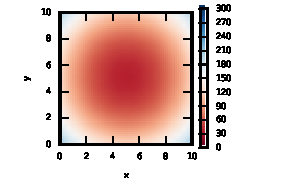
\includegraphics[width=\textwidth]{100IR4DTradPurspurscolorplot99}
	\caption{100 Iterations}
	\label{100IR4DTPCP99}
\end{subfigure}
\caption{State cost evolution when evader is at (5,5)}
\label{100IR4DTPCP}
\end{figure}

After the pursuer value iteration is run for a hundred iterations, the evader value iteration is also run for a hundred iterations with the updated pursuer cost, $J^{(100,1)}_p$. Just like with the pursuer value iteration, it took approximately 90 minutes to run one hundred iterations of evader value iteration, \Cref{4DVIrt}. The evolution of the evader state cost can be seen  in \Cref{100IR4DTECP}. Take note of the minimal difference in the state cost between ten and a hundred iterations. Notice that the average norm converges to the optimal average norm, \Cref{100IR4DTEnp}, and the difference between the average norm decreases exponentially fast, \Cref{100IR4DTEdnp}. Notice that despite maximizing over the same cost function, the average norm converges to approximately the same value as in \Cref{100IR4DTnp}.
\begin{figure}[h!]
\centering
\begin{subfigure}[t]{0.475\textwidth}
	\centering
	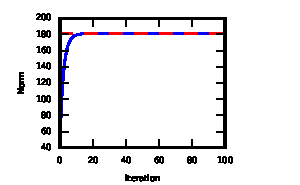
\includegraphics[width=\textwidth]{100IR4DTradEvadnormplot}
	\caption{Average norm of the evader state cost with red dashed line as the average norm of the optimal value}
	\label{100IR4DTEnp}
\end{subfigure}
\hfill
\begin{subfigure}[t]{0.475\textwidth}
	\centering
	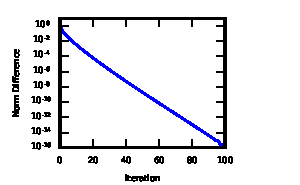
\includegraphics[width=\textwidth]{100IR4DTradEvaddiffNormplot}
	\caption{Normalized difference in average norm between sequential evader state costs}
	\label{100IR4DTEdnp}
\end{subfigure}
\caption{Diagnostic results of running 100 Iterations of Evader Value Iteration}
\label{100IR4DTEdiag}
\end{figure}  
\begin{figure}
\centering
\begin{subfigure}[b]{0.475\textwidth}
	\centering
	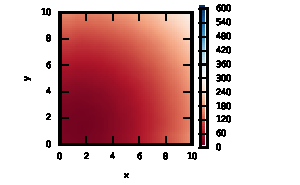
\includegraphics[width=\textwidth]{100IR4DTradEvadevadcolorplot0}
	\caption{1 Iteration }
	\label{100IR4DTECP0}
\end{subfigure}
\hfill
\begin{subfigure}[b]{0.475\textwidth}
	\centering
	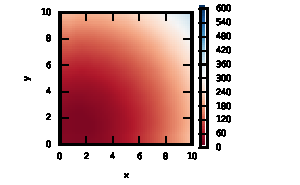
\includegraphics[width=\textwidth]{100IR4DTradEvadevadcolorplot1}
	\caption{2 Iterations}
	\label{100IR4DTECP1}
\end{subfigure}
\vskip\baselineskip
\begin{subfigure}[b]{0.475\textwidth}
	\centering
	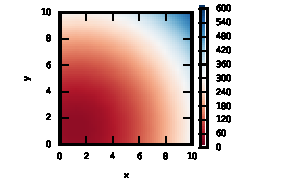
\includegraphics[width=\textwidth]{100IR4DTradEvadevadcolorplot9}
	\caption{10 Iterations}
	\label{100IR4DTECP9}
\end{subfigure}
\quad
\begin{subfigure}[b]{0.475\textwidth}
	\centering
	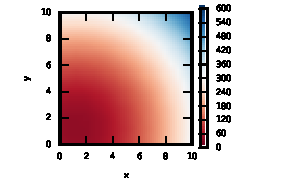
\includegraphics[width=\textwidth]{100IR4DTradEvadevadcolorplot99}
	\caption{100 Iterations}
	\label{100IR4DTECP99}
\end{subfigure}
\caption{State cost evolution when pursuer is at (1,1)}
\label{100IR4DTECP}
\end{figure}
\begin{table}
\caption{Value Iteration Program Run Times(sec)}
\label{4DVIrt}
\begin{center}
\begin{tabular}{||r|c|c||}\hline
  & 1 Iteration & 100 Iterations \\\hline
Pursuit & 57.6885 & 5942.2932 \\\hline
Evasion & 58.3154 & 5865.4880 \\\hline
\end{tabular}
\end{center}
\end{table}

Traditional value iteration was also implemented with \Cref{DPBRalg}. This algorithm was ran twice, once at $\Delta_{max} = 10^{-2}$ and $\delta_{max} = 10^{-2}$ for an equal comparison with the BR-TT-VI algorithm  and once where $\Delta_{max} = 10^{-5}$ and $\delta_{max} = 10^{-5}$ to determine optimality to a point where changes in the state cost were no longer noticeable. For the $(\Delta_{max} = 10^{-2},\delta_{max} = 10^{-2})$ case, on the first best response run both the pursuer and evader state costs converge to an average norm of 179 in about 10 iterations as can be seen by the blue line in \Cref{BR4DTSPnp,BR4DTSEnp}. Changes to the control on this run are minor enough that there are no major changes in state costs on the second run as can be seen by the red line segment in the same figures. This causes the algorithm to end after only two runs. To run the entire algorithm it took almost twenty minutes, \Cref{BRPRun}. 
\begin{figure}[h!]
\centering
\begin{subfigure}[t]{0.475\textwidth}
	\centering
	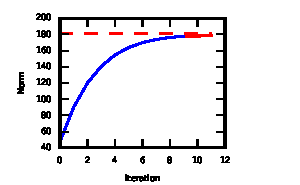
\includegraphics[width=\textwidth]{BR4DTSPursnormplot}
	\caption{Average norm of the pursuer state cost with red dashed line as the average norm of the optimal value}
	\label{BR4DTSPnp}
\end{subfigure}
\hfill
\begin{subfigure}[t]{0.475\textwidth}
	\centering
	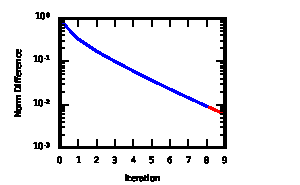
\includegraphics[width=\textwidth]{BR4DTSPursdiffNormplot}
	\caption{Normalized difference in average norm between sequential pursuer state costs}
	\label{BR4DTSPdnp}
\end{subfigure}
\caption{Pursuer diagnostic results of running Best Response Value Iteration Algorithm with $(\Delta_{max} = 10^{-2},\delta_{max} = 10^{-2})$. Blue solid line is the first run, while the red solid line is the second run}
\label{BR4DTSPdiag}
\end{figure}
\begin{figure}[h!]
\centering
\begin{subfigure}[t]{0.475\textwidth}
	\centering
	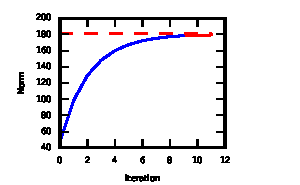
\includegraphics[width=\textwidth]{BR4DTSEvadnormplot}
	\caption{Average norm of the evader state cost with red dashed line as the average norm of the optimal value}
	\label{BR4DTSEnp}
\end{subfigure}
\hfill
\begin{subfigure}[t]{0.475\textwidth}
	\centering
	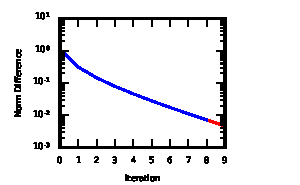
\includegraphics[width=\textwidth]{BR4DTSEvaddiffNormplot}
	\caption{Normalized difference in average norm between sequential evader state costs}
	\label{BR4DTSEdnp}
\end{subfigure}
\caption{Evader diagnostic results of running Best Response Value Iteration Algorithm with $(\Delta_{max} = 10^{-2},\delta_{max} = 10^{-2})$. Blue solid line is the first run, while the red solid line is the second run}
\label{BR4DTSEdiag}
\end{figure}

The pursuer state costs monotonically decrease toward the evaders position, \Cref{BR4DTSPcp}, while the evader's state costs monotonically decrease toward the pursuers position,\Cref{BR4DTSEcp}. The game was simulated with the pursuer starting at eight different positions and the evader starting at (5,5) as can be seen in \Cref{BR4DTSGp}. In each of these cases, the pursuer heads directly toward the evader while the evader heads in the opposite direct of the pursuer. Due to the pursuers faster speed in both the x and y axis, the distance between the pursuer and evader decreases directly to the origin, \Cref{BR4DTSGr}. It should be noted that due to the separation of the dynamics in the x and y axis, when the pursuer and evader have the same value on only one axis an oscillation occurs. This is due to the evader randomly darting to one or the other direction with the pursuer quickly following and overcoming the evader.
\begin{figure}[h!]
\centering
\begin{subfigure}[t]{0.475\textwidth}
	\centering
	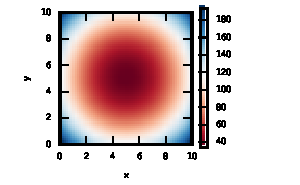
\includegraphics[width=\textwidth]{BR4DTSPurspurscolorplot}
	\caption{Pursuer state cost when evader is at (5,5)}
	\label{BR4DTSPcp}
\end{subfigure}
\hfill
\begin{subfigure}[t]{0.475\textwidth}
	\centering
	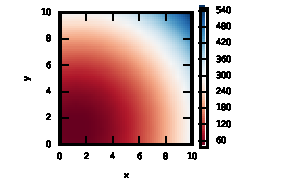
\includegraphics[width=\textwidth]{BR4DTSEvadevadcolorplot}
	\caption{Evader state cost when pursuer is at (1,1)}
	\label{BR4DTSEcp}
\end{subfigure}
\caption{State Costs after running Best Response Value Iteration Algorithm with $(\Delta_{max} = 10^{-2},\delta_{max} = 10^{-2})$}
\label{BR4DTScp}
\end{figure}
\begin{figure}
\centering
\begin{subfigure}[b]{0.3\textwidth}
	\centering
	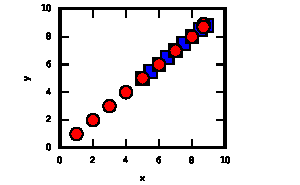
\includegraphics[width=\textwidth]{BR4DTSGamephaseplot1}
	\caption{(1,1) }
	\label{BR4DTSGp1}
\end{subfigure}
\hfill
\begin{subfigure}[b]{0.3\textwidth}
	\centering
	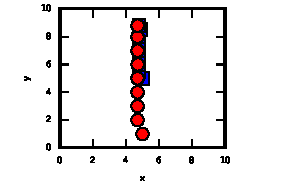
\includegraphics[width=\textwidth]{BR4DTSGamephaseplot2}
	\caption{(5,1)}
	\label{BR4DTSGp2}
\end{subfigure}
\hfill
\begin{subfigure}[b]{0.3\textwidth}
	\centering
	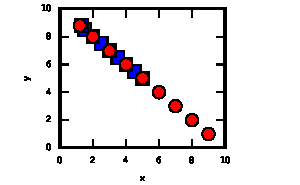
\includegraphics[width=\textwidth]{BR4DTSGamephaseplot3}
	\caption{(9,1)}
	\label{BR4DTSGp3}
\end{subfigure}
\vskip\baselineskip
\begin{subfigure}[b]{0.3\textwidth}
	\centering
	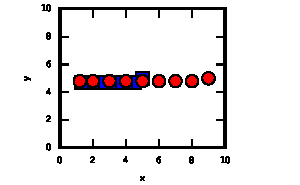
\includegraphics[width=\textwidth]{BR4DTSGamephaseplot4}
	\caption{(9,5) }
	\label{BR4DTSGp4}
\end{subfigure}
\hfill
\begin{subfigure}[b]{0.3\textwidth}
	\centering
	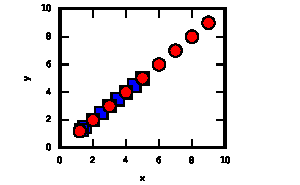
\includegraphics[width=\textwidth]{BR4DTSGamephaseplot5}
	\caption{(9,9)}
	\label{BR4DTSGp5}
\end{subfigure}
\hfill
\begin{subfigure}[b]{0.3\textwidth}
	\centering
	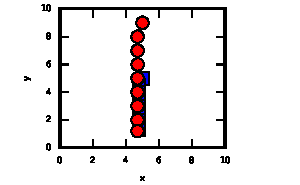
\includegraphics[width=\textwidth]{BR4DTSGamephaseplot6}
	\caption{(5,9)}
	\label{BR4DTSGp6}
\end{subfigure}
\vskip\baselineskip
\begin{subfigure}[b]{0.3\textwidth}
	\centering
	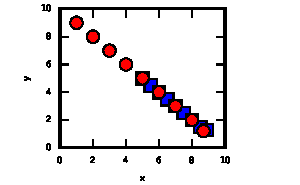
\includegraphics[width=\textwidth]{BR4DTSGamephaseplot7}
	\caption{(1,9) }
	\label{BR4DTSGp7}
\end{subfigure}
\quad
\begin{subfigure}[b]{0.3\textwidth}
	\centering
	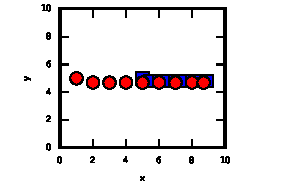
\includegraphics[width=\textwidth]{BR4DTSGamephaseplot8}
	\caption{(1,5)}
	\label{BR4DTSGp8}
\end{subfigure}
\caption{Pursuit-Evasion game with evader at (5,5) and pursuer at varying positions. 1 second intervals are used between each marker}
\label{BR4DTSGp}
\end{figure}
\begin{figure}
\centering
\begin{subfigure}[b]{0.3\textwidth}
	\centering
	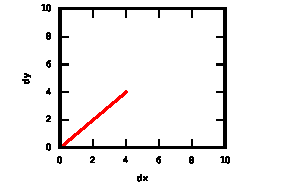
\includegraphics[width=\textwidth]{BR4DTSGamerelplot1}
	\caption{(1,1) }
	\label{BR4DTSGr1}
\end{subfigure}
\hfill
\begin{subfigure}[b]{0.3\textwidth}
	\centering
	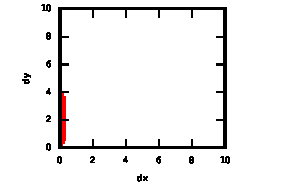
\includegraphics[width=\textwidth]{BR4DTSGamerelplot2}
	\caption{(5,1)}
	\label{BR4DTSGr2}
\end{subfigure}
\hfill
\begin{subfigure}[b]{0.3\textwidth}
	\centering
	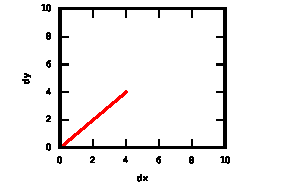
\includegraphics[width=\textwidth]{BR4DTSGamerelplot3}
	\caption{(9,1)}
	\label{BR4DTSGr3}
\end{subfigure}
\vskip\baselineskip
\begin{subfigure}[b]{0.3\textwidth}
	\centering
	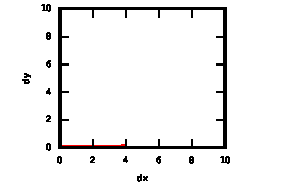
\includegraphics[width=\textwidth]{BR4DTSGamerelplot4}
	\caption{(9,5) }
	\label{BR4DTSGr4}
\end{subfigure}
\hfill
\begin{subfigure}[b]{0.3\textwidth}
	\centering
	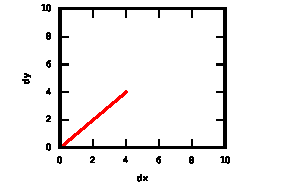
\includegraphics[width=\textwidth]{BR4DTSGamerelplot5}
	\caption{(9,9)}
	\label{BR4DTSGr5}
\end{subfigure}
\hfill
\begin{subfigure}[b]{0.3\textwidth}
	\centering
	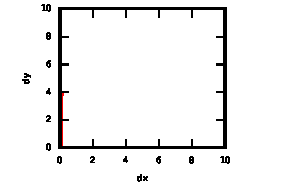
\includegraphics[width=\textwidth]{BR4DTSGamerelplot6}
	\caption{(5,9)}
	\label{BR4DTSGr6}
\end{subfigure}
\vskip\baselineskip
\begin{subfigure}[b]{0.3\textwidth}
	\centering
	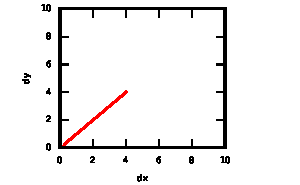
\includegraphics[width=\textwidth]{BR4DTSGamerelplot7}
	\caption{(1,9) }
	\label{BR4DTSGr7}
\end{subfigure}
\quad
\begin{subfigure}[b]{0.3\textwidth}
	\centering
	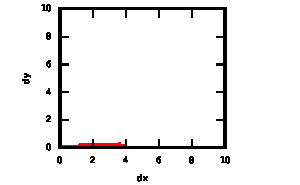
\includegraphics[width=\textwidth]{BR4DTSGamerelplot8}
	\caption{(1,5)}
	\label{BR4DTSGr8}
\end{subfigure}
\caption{Relative position of pursuer and evader in pursuit-Evasion game with evader at (5,5) and pursuer at varying positions}
\label{BR4DTSGr}
\end{figure}

A $(\Delta_{max} = 10^{-5},\delta_{max} = 10^{-5})$ case was also implemented to ensure that the $(\Delta_{max} = 10^{-2},\delta_{max} = 10^{-2})$ case ran to an appropriate termination. On the first best response run both the pursuer and evader state costs converge to an average norm of 180.97 in just over 25 iterations as seen by the blue solid line in \Cref{BR4DTCPnp,BR4DTCEnp}. The second run of best response again produces no notable change in the state cost of either the pursuer or the evader as seen by the red solid line in the same figures. Because of this the average norm of 180.97 will be considered optimal for the four-dimensional problem. In order to get this more accurate response, the algorithm ran for almost an hour, \Cref{BRPRun}. Despite the much longer run time, the results of the pursuit-evasion game do not noticeably change as can be seen by \Cref{BR4DTCcp,BR4DTCGp,BR4DTCGr} mirroring \Cref{BR4DTScp,BR4DTSGp,BR4DTSGr}. 
\begin{figure}[h!]
\centering
\begin{subfigure}[t]{0.475\textwidth}
	\centering
	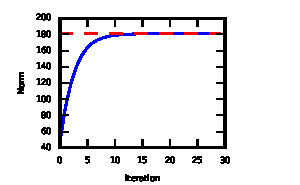
\includegraphics[width=\textwidth]{BR4DTCPursnormplot}
	\caption{Average norm of the pursuer state cost with red dashed line as the average norm of the optimal value}
	\label{BR4DTCPnp}
\end{subfigure}
\hfill
\begin{subfigure}[t]{0.475\textwidth}
	\centering
	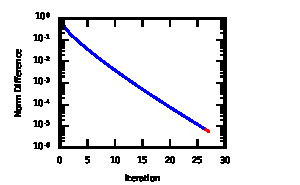
\includegraphics[width=\textwidth]{BR4DTCPursdiffNormplot}
	\caption{Normalized difference in average norm between sequential pursuer state costs}
	\label{BR4DTCPdnp}
\end{subfigure}
\caption{Pursuer diagnostic results of running Best Response Value Iteration Algorithm with $(\Delta_{max} = 10^{-5},\delta_{max} = 10^{-5})$. Blue solid line is the first run, while the red solid line is the second run}
\label{BR4DTCPdiag}
\end{figure}
\begin{figure}[h!]
\centering
\begin{subfigure}[t]{0.475\textwidth}
	\centering
	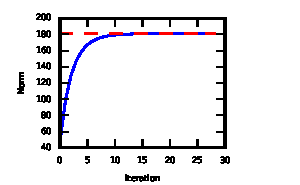
\includegraphics[width=\textwidth]{BR4DTCEvadnormplot}
	\caption{Average norm of the evader state cost with red dashed line as the average norm of the optimal value}
	\label{BR4DTCEnp}
\end{subfigure}
\hfill
\begin{subfigure}[t]{0.475\textwidth}
	\centering
	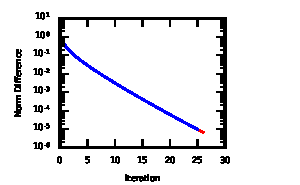
\includegraphics[width=\textwidth]{BR4DTCEvaddiffNormplot}
	\caption{Normalized difference in average norm between sequential evader state costs}
	\label{BR4DTCEdnp}
\end{subfigure}
\caption{Evader diagnostic results of running Best Response Value Iteration Algorithm with $(\Delta_{max} = 10^{-5},\delta_{max} = 10^{-5})$. Blue solid line is the first run, while the red solid line is the second run}
\label{BR4DTCEdiag}
\end{figure}
\begin{figure}[h!]
\centering
\begin{subfigure}[t]{0.475\textwidth}
	\centering
	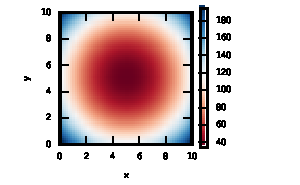
\includegraphics[width=\textwidth]{BR4DTCPurspurscolorplot}
	\caption{Pursuer state cost when evader is at (5,5)}
	\label{BR4DTCPcp}
\end{subfigure}
\hfill
\begin{subfigure}[t]{0.475\textwidth}
	\centering
	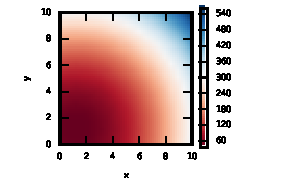
\includegraphics[width=\textwidth]{BR4DTCEvadevadcolorplot}
	\caption{Evader state cost when pursuer is at (1,1)}
	\label{BR4DTCEcp}
\end{subfigure}
\caption{State Costs after running Best Response Value Iteration Algorithm with $(\Delta_{max} = 10^{-5},\delta_{max} = 10^{-5})$}
\label{BR4DTCcp}
\end{figure}
\begin{figure}
\centering
\begin{subfigure}[b]{0.3\textwidth}
	\centering
	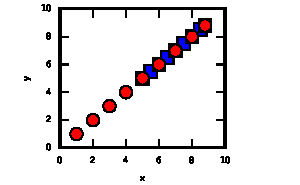
\includegraphics[width=\textwidth]{BR4DTCGamephaseplot1}
	\caption{(1,1) }
	\label{BR4DTCGp1}
\end{subfigure}
\hfill
\begin{subfigure}[b]{0.3\textwidth}
	\centering
	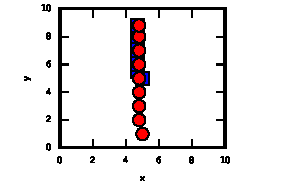
\includegraphics[width=\textwidth]{BR4DTCGamephaseplot2}
	\caption{(5,1)}
	\label{BR4DTCGp2}
\end{subfigure}
\hfill
\begin{subfigure}[b]{0.3\textwidth}
	\centering
	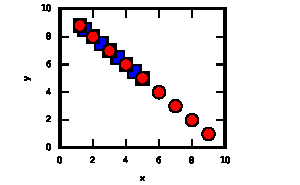
\includegraphics[width=\textwidth]{BR4DTCGamephaseplot3}
	\caption{(9,1)}
	\label{BR4DTCGp3}
\end{subfigure}
\vskip\baselineskip
\begin{subfigure}[b]{0.3\textwidth}
	\centering
	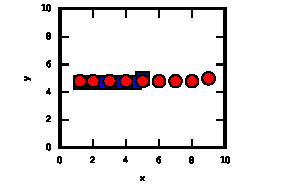
\includegraphics[width=\textwidth]{BR4DTCGamephaseplot4}
	\caption{(9,5) }
	\label{BR4DTCGp4}
\end{subfigure}
\hfill
\begin{subfigure}[b]{0.3\textwidth}
	\centering
	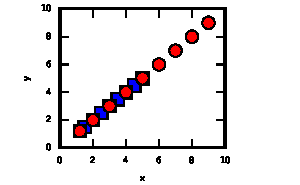
\includegraphics[width=\textwidth]{BR4DTCGamephaseplot5}
	\caption{(9,9)}
	\label{BR4DTCGp5}
\end{subfigure}
\hfill
\begin{subfigure}[b]{0.3\textwidth}
	\centering
	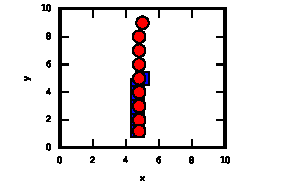
\includegraphics[width=\textwidth]{BR4DTCGamephaseplot6}
	\caption{(5,9)}
	\label{BR4DTCGp6}
\end{subfigure}
\vskip\baselineskip
\begin{subfigure}[b]{0.3\textwidth}
	\centering
	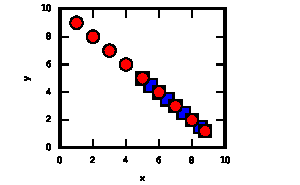
\includegraphics[width=\textwidth]{BR4DTCGamephaseplot7}
	\caption{(1,9) }
	\label{BR4DTCGp7}
\end{subfigure}
\quad
\begin{subfigure}[b]{0.3\textwidth}
	\centering
	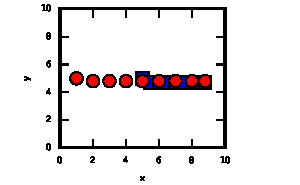
\includegraphics[width=\textwidth]{BR4DTCGamephaseplot8}
	\caption{(1,5)}
	\label{BR4DTCGp8}
\end{subfigure}
\caption{Pursuit-Evasion game with evader at (5,5) and pursuer at varying positions. 1 second intervals are used between each marker}
\label{BR4DTCGp}
\end{figure}
\begin{figure}
\centering
\begin{subfigure}[b]{0.3\textwidth}
	\centering
	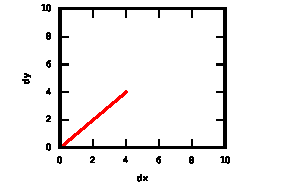
\includegraphics[width=\textwidth]{BR4DTCGamerelplot1}
	\caption{(1,1) }
	\label{BR4DTCGr1}
\end{subfigure}
\hfill
\begin{subfigure}[b]{0.3\textwidth}
	\centering
	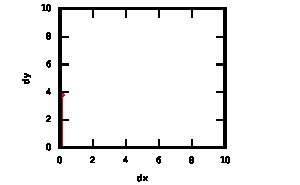
\includegraphics[width=\textwidth]{BR4DTCGamerelplot2}
	\caption{(5,1)}
	\label{BR4DTCGr2}
\end{subfigure}
\hfill
\begin{subfigure}[b]{0.3\textwidth}
	\centering
	\includegraphics[width=\textwidth]{BR4DTCGamerelplot3}
	\caption{(9,1)}
	\label{BR4DTCGr3}
\end{subfigure}
\vskip\baselineskip
\begin{subfigure}[b]{0.3\textwidth}
	\centering
	\includegraphics[width=\textwidth]{BR4DTCGamerelplot4}
	\caption{(9,5) }
	\label{BR4DTCGr4}
\end{subfigure}
\hfill
\begin{subfigure}[b]{0.3\textwidth}
	\centering
	\includegraphics[width=\textwidth]{BR4DTCGamerelplot5}
	\caption{(9,9)}
	\label{BR4DTCGr5}
\end{subfigure}
\hfill
\begin{subfigure}[b]{0.3\textwidth}
	\centering
	\includegraphics[width=\textwidth]{BR4DTCGamerelplot6}
	\caption{(5,9)}
	\label{BR4DTCGr6}
\end{subfigure}
\vskip\baselineskip
\begin{subfigure}[b]{0.3\textwidth}
	\centering
	\includegraphics[width=\textwidth]{BR4DTCGamerelplot7}
	\caption{(1,9) }
	\label{BR4DTCGr7}
\end{subfigure}
\quad
\begin{subfigure}[b]{0.3\textwidth}
	\centering
	\includegraphics[width=\textwidth]{BR4DTCGamerelplot8}
	\caption{(1,5)}
	\label{BR4DTCGr8}
\end{subfigure}
\caption{Relative position of pursuer and evader in pursuit-Evasion game with evader at (5,5) and pursuer at varying positions}
\label{BR4DTCGr}
\end{figure}             

\subsection{Tensor-Train-Decomposition-Based Value Iteration}
Tensor-Train-Decomposition-Based Value Iteration(TT-VI) can also be used to solve the pursuit-evasion game with simple Euclidean dynamics. Just as with VI, before running \Cref{BRTVIalg} both the pursuer and evader TT-VI were run for 100 iterations to characterize the algorithm when run past completion. Once again both the pursuer and evader state cost were set to initialized such that $J^{(0,0)}_p(z_i) = (x_1-x_2)^2+(y_1-y_2)^2$ and $J^{(0,0)}_e(z_i) = (x_1-x_2)^2+(y_1-y_2)^2$. The pursuer TT-VI is run first for one hundred iterations. These one hundred iterations only take about eight minutes, \Cref{4DTTVIrt}. The evolution of the pursuer state cost can be seen  in \Cref{100IR4DTVIPCP}. Once again there is very little difference between the state cost at ten iterations and a hundred iterations. Notice that the average norm converges to the optimal average norm, \Cref{100IR4DTVInp}. The difference between the average norm logarithmically decreases until a difference of about $10^{-3}$ at which point the plot fluctuates about this point \Cref{100IR4DTVIdnp}. Average tensor rank remains constant at 3.60, \Cref{100IR4DTVIrkp}, while the fraction of states used fluctuates between about 0.020 and 0.013 of the original $21^4$ states, \Cref{100IR4DTVIsp}. 
\begin{figure}[h!]
\centering
\begin{subfigure}[t]{0.475\textwidth}
	\centering
	\includegraphics[width=\textwidth]{100IR4DTVIPursnormplot}
	\caption{Average norm of the pursuer state cost with red dashed line as the average norm of the optimal value}
	\label{100IR4DTVInp}
\end{subfigure}
\hfill
\begin{subfigure}[t]{0.475\textwidth}
	\centering
	\includegraphics[width=\textwidth]{100IR4DTVIPursdiffNormplot}
	\caption{Normalized difference in average norm between sequential pursuer state costs}
	\label{100IR4DTVIdnp}
\end{subfigure}
\vskip\baselineskip
\begin{subfigure}[t]{0.475\textwidth}
	\centering
	\includegraphics[width=\textwidth]{100IR4DTVIPursRankplot}
	\caption{Average rank of the pursuer state cost tensor}
	\label{100IR4DTVIrkp}
\end{subfigure}
\hfill
\begin{subfigure}[t]{0.475\textwidth}
	\centering
	\includegraphics[width=\textwidth]{100IR4DTVIPurssizeplot}
	\caption{Fraction of states used for the pursuer state cost tensor}
	\label{100IR4DTVIsp}
\end{subfigure}
\caption{Diagnostic results of running 100 Iterations of Pursuit TT-VI}
\label{100IR4DTVIdiag}
\end{figure} 
\begin{figure}
\centering
\begin{subfigure}[b]{0.475\textwidth}
	\centering
	\includegraphics[width=\textwidth]{100IR4DTVIPurspurscolorplot0}
	\caption{1 Iteration }
	\label{100IR4DTVIPCP0}
\end{subfigure}
\hfill
\begin{subfigure}[b]{0.475\textwidth}
	\centering
	\includegraphics[width=\textwidth]{100IR4DTVIPurspurscolorplot1}
	\caption{2 Iterations}
	\label{100IR4DTVIPCP1}
\end{subfigure}
\vskip\baselineskip
\begin{subfigure}[b]{0.475\textwidth}
	\centering
	\includegraphics[width=\textwidth]{100IR4DTVIPurspurscolorplot9}
	\caption{10 Iterations}
	\label{100IR4DTVIPCP9}
\end{subfigure}
\quad
\begin{subfigure}[b]{0.475\textwidth}
	\centering
	\includegraphics[width=\textwidth]{100IR4DTVIPurspurscolorplot99}
	\caption{100 Iterations}
	\label{100IR4DTVIPCP99}
\end{subfigure}
\caption{State cost evolution when evader is at (5,5)}
\label{100IR4DTVIPCP}
\end{figure}

After the pursuer TT-VI is run for a hundred iterations, the evader TT-VI is run for a hundred iterations with the updated pursuer cost, $J^{(100,1)}_p$. Just like the pursuer TT-VI, the evader TT-VI only takes about eight minutes to complete a hundred iterations, \Cref{4DTTVIrt}. The evolution of the evader state cost can be seen  in \Cref{100IR4DTVIECP}. The average norm still converges to the optimal average norm, \Cref{100IR4DTVIEnp}. Just as with pursuer TT-VI the difference between the average norm logarithmically decreases until a difference of about $10^{-3}$ at which point the plot fluctuates about this point \Cref{100IR4DTVIEdnp}. Average tensor rank also remains constant at 3.60, \Cref{100IR4DTVIErkp}, while the fraction of states used fluctuates between about 0.020 and 0.013 of the original $21^4$ states, \Cref{100IR4DTVIEsp}. Just as with VI, the average norm converges to approximately the same value as in \Cref{100IR4DTVInp}.
\begin{figure}[h!]
\centering
\begin{subfigure}[t]{0.475\textwidth}
	\centering
	\includegraphics[width=\textwidth]{100IR4DTVIEvadnormplot}
	\caption{Average norm of the evader state cost with red dashed line as the average norm of the optimal value}
	\label{100IR4DTVIEnp}
\end{subfigure}
\hfill
\begin{subfigure}[t]{0.475\textwidth}
	\centering
	\includegraphics[width=\textwidth]{100IR4DTVIEvaddiffNormplot}
	\caption{Normalized difference in average norm between sequential evader state costs}
	\label{100IR4DTVIEdnp}
\end{subfigure}
\vskip\baselineskip
\begin{subfigure}[t]{0.475\textwidth}
	\centering
	\includegraphics[width=\textwidth]{100IR4DTVIEvadRankplot}
	\caption{Average rank of the evader state cost tensor}
	\label{100IR4DTVIErkp}
\end{subfigure}
\hfill
\begin{subfigure}[t]{0.475\textwidth}
	\centering
	\includegraphics[width=\textwidth]{100IR4DTVIEvadsizeplot}
	\caption{Fraction of states used for the evader state cost tensor}
	\label{100IR4DTVIEsp}
\end{subfigure}
\caption{Diagnostic results of running 100 Iterations of Evade TVI}
\label{100IR4DTVIEdiag}
\end{figure} 
\begin{figure}
\centering
\begin{subfigure}[b]{0.475\textwidth}
	\centering
	\includegraphics[width=\textwidth]{100IR4DTVIEvadevadcolorplot0}
	\caption{1 Iteration }
	\label{100IR4DTVIECP0}
\end{subfigure}
\hfill
\begin{subfigure}[b]{0.475\textwidth}
	\centering
	\includegraphics[width=\textwidth]{100IR4DTVIEvadevadcolorplot1}
	\caption{2 Iterations}
	\label{100IR4DTVIECP1}
\end{subfigure}
\vskip\baselineskip
\begin{subfigure}[b]{0.475\textwidth}
	\centering
	\includegraphics[width=\textwidth]{100IR4DTVIEvadevadcolorplot9}
	\caption{10 Iterations}
	\label{100IR4DTVIECP9}
\end{subfigure}
\quad
\begin{subfigure}[b]{0.475\textwidth}
	\centering
	\includegraphics[width=\textwidth]{100IR4DTVIEvadevadcolorplot99}
	\caption{100 Iterations}
	\label{100IR4DTVIECP99}
\end{subfigure}
\caption{State cost evolution when pursuer is at (1,1)}
\label{100IR4DTVIECP}
\end{figure}
\begin{table}
\caption{4D TT-VI Program Run Times(sec)}
\label{4DTTVIrt}
\begin{center}
\begin{tabular}{||r|c|c||}\hline
  & 1 Iteration & 100 Iterations \\\hline
Pursuit & 4.3525 & 473.1945 \\\hline
Evasion & 4.6160 & 483.1202 \\\hline
\end{tabular}
\end{center}
\end{table}

The four-dimensional problem was also solved using \Cref{BRTVIalg}. $\Delta_{max} = 10^{-2}$ and $\delta_{max} = 10^{-2}$ were used as the best response and the value iteration accuracy respectively. On the first best response run both the pursuer and evader state costs converge to an average norm of 179 in about 10 iterations as can be seen by the solid blue line in \Cref{BR4DTVIPnp,BR4DTVIEnp}. The average rank for both the pursuer and evader stays at 3.6 throughout, \Cref{BR4DTVIPrkp,BR4DTVIErkp}. In determining the new state costs, less than $1/50$ of the total states is used for each iteration of TT-VI, \Cref{BR4DTVIPsp,BR4DTVIEsp}. On the second run of best response, the changes remain minor resulting in virtually no change to the norm, rank, or states used for both the pursuer and the evader as can be seen by the solid red line in the previous figures, \Cref{BR4DTVIPdiag,BR4DTVIEdiag}. The entire BR-TT-VI algorithm for the four-dimensional problem takes less than two minutes to complete, \Cref{BRPRun}. 
\begin{figure}[h!]
\centering
\begin{subfigure}[t]{0.475\textwidth}
	\centering
	\includegraphics[width=\textwidth]{BR4DTVIPursnormplot}
	\caption{Average norm of the pursuer state cost with red dashed line as the average norm of the optimal value}
	\label{BR4DTVIPnp}
\end{subfigure}
\hfill
\begin{subfigure}[t]{0.475\textwidth}
	\centering
	\includegraphics[width=\textwidth]{BR4DTVIPursdiffNormplot}
	\caption{Normalized difference in average norm between sequential pursuer state costs}
	\label{BR4DTVIPdnp}
\end{subfigure}
\vskip\baselineskip
\begin{subfigure}[t]{0.475\textwidth}
	\centering
	\includegraphics[width=\textwidth]{BR4DTVIPursRankplot}
	\caption{Average rank of the pursuer state cost tensor}
	\label{BR4DTVIPrkp}
\end{subfigure}
\hfill
\begin{subfigure}[t]{0.475\textwidth}
	\centering
	\includegraphics[width=\textwidth]{BR4DTVIPurssizeplot}
	\caption{Fraction of states used for the pursuer state cost tensor}
	\label{BR4DTVIPsp}
\end{subfigure}
\caption{Pursuer diagnostic results of running BR-TT-VI Algorithm with $(\Delta_{max} = 10^{-2},\delta_{max} = 10^{-2})$. Blue solid line is the first run, while the red solid line is the second run}
\label{BR4DTVIPdiag}
\end{figure}
\begin{figure}[h!]
\centering
\begin{subfigure}[t]{0.475\textwidth}
	\centering
	\includegraphics[width=\textwidth]{BR4DTVIEvadnormplot}
	\caption{Average norm of the evader state cost with red dashed line as the average norm of the optimal value}
	\label{BR4DTVIEnp}
\end{subfigure}
\hfill
\begin{subfigure}[t]{0.475\textwidth}
	\centering
	\includegraphics[width=\textwidth]{BR4DTVIEvaddiffNormplot}
	\caption{Normalized difference in average norm between sequential evader state costs}
	\label{BR4DTVIEdnp}
\end{subfigure}
\vskip\baselineskip
\begin{subfigure}[t]{0.475\textwidth}
	\centering
	\includegraphics[width=\textwidth]{BR4DTVIEvadRankplot}
	\caption{Average rank of the evader state cost tensor}
	\label{BR4DTVIErkp}
\end{subfigure}
\hfill
\begin{subfigure}[t]{0.475\textwidth}
	\centering
	\includegraphics[width=\textwidth]{BR4DTVIEvadsizeplot}
	\caption{Fraction of states used for the evader state cost tensor}
	\label{BR4DTVIEsp}
\end{subfigure}
\caption{Evader diagnostic results of running Best Response TVI Algorithm with $(\Delta_{max} = 10^{-2},\delta_{max} = 10^{-2})$. Blue solid line is the first run, while the red solid line is the second run}
\label{BR4DTVIEdiag}
\end{figure}

The pursuer state costs monotonically decrease toward the evaders position, \Cref{BR4DTVIPcp}, while the evader's state costs monotonically decrease toward the pursuers position, \Cref{BR4DTVIEcp}. The pursuer heads directly towards the evader, while the evader heads in the opposite direction of the pursuer as can be seen in \Cref{BR4DTVIp}. Due to the pursuer's greater speed, the game has the pursuer constantly decreasing the distance between itself and the evader until capture as can be seen in \Cref{BR4DTVIr}.
\begin{figure}[h!]
\centering
\begin{subfigure}[t]{0.475\textwidth}
	\centering
	\includegraphics[width=\textwidth]{BR4DTVIPurspurscolorplot}
	\caption{Pursuer state cost when evader is at (5,5)}
	\label{BR4DTVIPcp}
\end{subfigure}
\hfill
\begin{subfigure}[t]{0.475\textwidth}
	\centering
	\includegraphics[width=\textwidth]{BR4DTVIEvadevadcolorplot}
	\caption{Evader state cost when pursuer is at (1,1)}
	\label{BR4DTVIEcp}
\end{subfigure}
\caption{State Costs after running BR-TT-VI Algorithm with $(\Delta_{max} = 10^{-2},\delta_{max} = 10^{-2})$}
\label{BR4DTVIcp}
\end{figure}
\begin{figure}
\centering
\begin{subfigure}[b]{0.3\textwidth}
	\centering
	\includegraphics[width=\textwidth]{BR4DTVIphaseplot1}
	\caption{(1,1) }
	\label{BR4DTVIp1}
\end{subfigure}
\hfill
\begin{subfigure}[b]{0.3\textwidth}
	\centering
	\includegraphics[width=\textwidth]{BR4DTVIphaseplot2}
	\caption{(5,1)}
	\label{BR4DTVIp2}
\end{subfigure}
\hfill
\begin{subfigure}[b]{0.3\textwidth}
	\centering
	\includegraphics[width=\textwidth]{BR4DTVIphaseplot3}
	\caption{(9,1)}
	\label{BR4DTVIp3}
\end{subfigure}
\vskip\baselineskip
\begin{subfigure}[b]{0.3\textwidth}
	\centering
	\includegraphics[width=\textwidth]{BR4DTVIphaseplot4}
	\caption{(9,5) }
	\label{BR4DTVIp4}
\end{subfigure}
\hfill
\begin{subfigure}[b]{0.3\textwidth}
	\centering
	\includegraphics[width=\textwidth]{BR4DTVIphaseplot5}
	\caption{(9,9)}
	\label{BR4DTVIp5}
\end{subfigure}
\hfill
\begin{subfigure}[b]{0.3\textwidth}
	\centering
	\includegraphics[width=\textwidth]{BR4DTVIphaseplot6}
	\caption{(5,9)}
	\label{BR4DTVIp6}
\end{subfigure}
\vskip\baselineskip
\begin{subfigure}[b]{0.3\textwidth}
	\centering
	\includegraphics[width=\textwidth]{BR4DTVIphaseplot7}
	\caption{(1,9) }
	\label{BR4DTVIp7}
\end{subfigure}
\quad
\begin{subfigure}[b]{0.3\textwidth}
	\centering
	\includegraphics[width=\textwidth]{BR4DTVIphaseplot8}
	\caption{(1,5)}
	\label{BR4DTVIp8}
\end{subfigure}
\caption{Pursuit-Evasion game with evader at (5,5) and pursuer at varying positions. 1 second intervals are used between each marker}
\label{BR4DTVIp}
\end{figure}
\begin{figure}
\centering
\begin{subfigure}[b]{0.3\textwidth}
	\centering
	\includegraphics[width=\textwidth]{BR4DTVIrelplot1}
	\caption{(1,1) }
	\label{BR4DTVIr1}
\end{subfigure}
\hfill
\begin{subfigure}[b]{0.3\textwidth}
	\centering
	\includegraphics[width=\textwidth]{BR4DTVIrelplot2}
	\caption{(5,1)}
	\label{BR4DTVIr2}
\end{subfigure}
\hfill
\begin{subfigure}[b]{0.3\textwidth}
	\centering
	\includegraphics[width=\textwidth]{BR4DTVIrelplot3}
	\caption{(9,1)}
	\label{BR4DTVIr3}
\end{subfigure}
\vskip\baselineskip
\begin{subfigure}[b]{0.3\textwidth}
	\centering
	\includegraphics[width=\textwidth]{BR4DTVIrelplot4}
	\caption{(9,5) }
	\label{BR4DTVIr4}
\end{subfigure}
\hfill
\begin{subfigure}[b]{0.3\textwidth}
	\centering
	\includegraphics[width=\textwidth]{BR4DTVIrelplot5}
	\caption{(9,9)}
	\label{BR4DTVIr5}
\end{subfigure}
\hfill
\begin{subfigure}[b]{0.3\textwidth}
	\centering
	\includegraphics[width=\textwidth]{BR4DTVIrelplot6}
	\caption{(5,9)}
	\label{BR4DTVIr6}
\end{subfigure}
\vskip\baselineskip
\begin{subfigure}[b]{0.3\textwidth}
	\centering
	\includegraphics[width=\textwidth]{BR4DTVIrelplot7}
	\caption{(1,9) }
	\label{BR4DTVIr7}
\end{subfigure}
\quad
\begin{subfigure}[b]{0.3\textwidth}
	\centering
	\includegraphics[width=\textwidth]{BR4DTVIrelplot8}
	\caption{(1,5)}
	\label{BR4DTVIr8}
\end{subfigure}
\caption{Relative position of pursuer and evader in pursuit-Evasion game with evader at (5,5) and pursuer at varying positions}
\label{BR4DTVIr}
\end{figure}     

\subsection{Comparison of Traditional Value Iteration and TT-VI}
Both VI and TT-VI can be used to solve the four-dimensional simple euclidean dynamics problem, however each method has its advantages and drawbacks. For the four-dimensional pursuit-evasion problem both VI and TT-VI successfully solve the problem. This can be seen by the nearly identical solutions from all eight starting positions for both the state cost results from VI and the state cost result from TT-VI as seen in \Cref{BR4DTSGp,BR4DTCGp,BR4DTVIp}. All average norms of the state costs also converge to the average norm of the optimal solution of 180.97, \Cref{BR4DTSPnp,BR4DTSEnp,BR4DTCPnp,BR4DTCEnp,BR4DTVIPnp,BR4DTVIEnp}. However, the precision of VI can be more exact than TT-VI. This can be seen in the difference between \Cref{100IR4DTdnp,100IR4DTEdnp} and \Cref{100IR4DTVIdnp,100IR4DTVIEdnp}. While the traditional value iteration continues to become more precise until limited by the precision of the variable (about $10^{-16}$), TVI is constrained in its precision by the accuracy of the tensor approximation (for the given example about $10^{-3}$). Furthermore, TVI can only tighten its precision at the potential expense in increased run time. 

Although traditional value iteration has benefits when it comes to precision, TT-VI can compute the solution more efficiently. Using the $10^{-2}$ error bounds, TT-VI runs more than ten times faster than the traditional method as can be seen in \Cref{4DVIrt,4DTTVIrt,BRPRun}. Use of the TT-VI algorithm also conserves memory. As seen in \Cref{4Dstore}, the state cost representations of TT-VI are approximately an eighth the size of the four-dimensional arrays used to store the state costs in VI. This four-dimensional example shows that TT-VI provides many benefits for problems already solvable by VI.
\begin{table}
\caption{State Cost Storage}
\label{4Dstore}
\begin{center}
\begin{tabular}{|r|c|c|}\hline
  & Value Iteration & TT-VI \\\hline
Pursuit & 8 MB & 883.3 kB \\\hline
Evasion & 8 MB & 1.1 MB \\\hline
\end{tabular}
\end{center}
\end{table}

\begin{table}
\caption{Best Response Program Run Times}
\label{BRPRun}
\begin{center}
\begin{tabular}{|r|c|c|c|c|}\hline
  & 4D VI($10^{-2}$) & 4D VI($10^{-5}$) & 4D BR-TT-VI($10^{-2}$) & 6D BR-TT-VI ($10^{-2}$)\\\hline
Time(s) & 1152.3172 & 3123.4174 & 102.0020 & 593.2975 \\\hline

\end{tabular}
\end{center}
\end{table}  

\section{Six-Dimensional Problem}
For the six dimensional problem, the pursuer and evader adapt Dubins car dynamics as outlined in \cite{dubins}.  The pursuer and evader remain in a $10 \times 10$ two-dimensional  state space with the addition of a heading state for both. The six dimensions are the $x$ position of the pursuer $x_1$, the $y$ position of the pursuer $y_1$, the heading of the pursuer $\theta_1$, the $x$ position of the evader $x_2$, the $y$ position of the evader $y_2$, and the heading of the evader $\theta_2$. This results in a state space such that $z_i = (x_1,y_1,\theta_1,x_2,y_2,\theta_2)$. Each of the dimensions are bounded as follows:
\begin{eqnarray*}
x_1 & \in & [0,10]\\
y_1 & \in & [0,10]\\
\theta_1 & \in & [0,2\pi]\\
x_2 & \in & [0,10]\\
y_2 & \in & [0,10]\\
\theta_2 & \in & [0,2\pi].
\end{eqnarray*} 
Both the pursuer and the evader have a single control for their change in heading, respectively $u_1$ and $u_2$. These controls are bounded between $[-\dfrac{\pi}{4},\dfrac{\pi}{4}]$. The pursuer and evader each have a constant velocity as defined by $V_1$ and $V_2$ respectively. For this problem $V_1 = 1$ and $V_2 = 0.5$. This results in the following system dynamics:
\begin{eqnarray}\label{eqns2}
\dot{x}_1 & = & x_1 +V_1cos(\theta_1)dt,\\
\dot{y}_1 & = & y_1 +V_1sin(\theta_1)dt,\\
\dot{\theta_1}  & = & \theta_1 + V_1tan(u_1)dt\\
\dot{x}_2 & = & x_2 +V_2cos(\theta_2)dt,\\
\dot{y}_2 & = & y_2 +V_2sin(\theta_2)dt,\\
\dot{\theta_2}  & = & \theta_2 + V_2tan(u_2)dt.
\end{eqnarray}
Each dimension is again discretized into 21 equally spaced states for a total of $21^6 \approx 9\cdot10^7$ discrete states. This discretization creates the same discrete state space as for the four-dimensional problem for the $x$ and $y$ states. The theta values are discretized such that the four cardinal directions are included and $0$ and $2\pi$ are redundantly kept in the discretization as can be seen:
\begin{eqnarray*}
\theta_1 & \in & [0,\dfrac{\pi}{10},\dfrac{\pi}{5},\dfrac{3\pi}{10},\dfrac{2\pi}{5},\dfrac{\pi}{2},\dfrac{3\pi}{5},\dfrac{7\pi}{10},\dfrac{4\pi}{5},\dfrac{9\pi}{10},\pi,\dfrac{11\pi}{10},\dfrac{6\pi}{5},\dfrac{13\pi}{10},\dfrac{7\pi}{5},\dfrac{3\pi}{2},\dfrac{8\pi}{5},\dfrac{17\pi}{10},\dfrac{9\pi}{5},\dfrac{19\pi}{10},2\pi]\\
\theta_2 & \in & [0,\dfrac{\pi}{10},\dfrac{\pi}{5},\dfrac{3\pi}{10},\dfrac{2\pi}{5},\dfrac{\pi}{2},\dfrac{3\pi}{5},\dfrac{7\pi}{10},\dfrac{4\pi}{5},\dfrac{9\pi}{10},\pi,\dfrac{11\pi}{10},\dfrac{6\pi}{5},\dfrac{13\pi}{10},\dfrac{7\pi}{5},\dfrac{3\pi}{2},\dfrac{8\pi}{5},\dfrac{17\pi}{10},\dfrac{9\pi}{5},\dfrac{19\pi}{10},2\pi].
\end{eqnarray*} 
Value iteration can also be used to solve for the optimal cost at each state. The problem is modeled as in \Cref{peprobdes}. A state cost function based on the distance between the pursuer and evader was chosen: 
\begin{equation}\label{6cost}
G(z_i,u_1,u_2)= 10+(x_1-x_2)^2+(y_1-y_2)^2.
\end{equation}
The constant of $10$ is added to provided a buffer for the BR-TT-VI approximation in order to prevent negative values. A discount factor of $\gamma = 0.7$ was chosen. Applying the state cost function and discount factor to \Cref{pbell} results in the update functions for the six-dimensional pursuit-evasion problem:
\begin{equation}\label{6pbell}
J_p^{(k+1,K)}(z_i)= \underset{u_1 }{\operatorname{min }}[10+(x_1-x_2)^2+(y_1-y_2)^2+0.7 J_p^{(k,K)}(z_j|z_i,u_1,u_2^K)],
\end{equation}
\begin{equation}\label{6ebell}
J_e^{(k+1,K)}(z_i)= \underset{u_2 }{\operatorname{max }}[10+(x_1-x_2)^2+(y_1-y_2)^2+0.7 J_e^{(k,K)}(z_j|z_i,u_1^K,u_2)].
\end{equation} 
By running \Cref{BRTVIalg} with \Cref{6pbell,6ebell} results in the given optimal value functions:
\begin{equation}\label{6pbropt}
J_p^{(*,*)}(z_i)= \underset{u_1 }{\operatorname{min }}[10+(x_1-x_2)^2+(y_1-y_2)^2+0.7 J_p^{(*,*)}(z_j|z_i,u_1,u_2^*)],
\end{equation}
\begin{equation}\label{6ebropt}
J_e^{(*,*)}(z_i)= \underset{u_2 }{\operatorname{max }}[10+(x_1-x_2)^2+(y_1-y_2)^2+0.7 J_e^{(*,*)}(z_j|z_i,u_1^*,u_2)].
\end{equation}    
These optimal value functions \ref{6pbropt} \ref{6ebropt} can be used to solve the following pursuit-evasion optimization problem:
\begin{eqnarray}\label{6opt}
&&\underset{u_1 }{\operatorname{min }}\underset{u_2 }{\operatorname{max }}[\int_{0}^{T}e^{-0.7t}(10+(x_1(t)-x_2(t))^2+(y_1(t)-y_2(t))^2)dt]\\
&\textnormal{s.t.}&\ref{eqns2}.
\end{eqnarray}

\subsection{Solving the Six-Dimensional Pursuit-Evasion Problem}
The excessive size of the six-dimensional pursuit-evasion game makes this problem hard to solve with traditional value iteration. One iteration of VI on the pursuit problem takes over thirteen hours to complete. However, BR-TT-VI may be used to solve the problem within some accuracy $\varepsilon$ in relatively short periods of time. Just as with the four-dimensional problem, before applying the BR-TT-VI algorithm a hundred iterations of the pursuer and evader TT-VI were conducted on the six-dimensional problem. 

Once again both the pursuer and evader state cost were set to initialized such that $J^{(0,0)}_p(z_i) = (x_1-x_2)^2+(y_1-y_2)^2$ and $J^{(0,0)}_e(z_i) = (x_1-x_2)^2+(y_1-y_2)^2$. The pursuer TT-VI is run first for one hundred iterations. These hundred iterations only took about fifty minutes which is less than half the time it took VI to run a hundred iterations of the four-dimensional pursuit problem, \Cref{6DTTVIrt}. The evolution of the pursuer state cost in relation to the x and y position of the pursuer can be seen  in \Cref{100IR6DTVIPCP}. Once again there is very little difference between the state cost at ten iterations and a hundred iterations. The average norm converges to a little over 180 as seen in \Cref{100IR6DTVInp}. The difference between the average norm logarithmically decreases until a difference of just over $10^{-3}$ at which point the plot fluctuates about this point, \Cref{100IR6DTVIdnp}. Average tensor rank starts at 3.85 but quickly jumps up to just below 4.3, \Cref{100IR6DTVIrkp}. Fluctuating at about 0.0001 of the original $21^6$ states, the fraction of states used is even smaller than in the four-dimensional problem, \Cref{100IR6DTVIsp}.
\begin{figure}[h!]
\centering
\begin{subfigure}[t]{0.475\textwidth}
	\centering
	\includegraphics[width=\textwidth]{100IR6DTVIPursnormplot}
	\caption{Average norm of the pursuer state cost}
	\label{100IR6DTVInp}
\end{subfigure}
\hfill
\begin{subfigure}[t]{0.475\textwidth}
	\centering
	\includegraphics[width=\textwidth]{100IR6DTVIPursdiffNormplot}
	\caption{Normalized difference in average norm between sequential pursuer state costs}
	\label{100IR6DTVIdnp}
\end{subfigure}
\vskip\baselineskip
\begin{subfigure}[t]{0.475\textwidth}
	\centering
	\includegraphics[width=\textwidth]{100IR6DTVIPursRankplot}
	\caption{Average rank of the pursuer state cost tensor}
	\label{100IR6DTVIrkp}
\end{subfigure}
\hfill
\begin{subfigure}[t]{0.475\textwidth}
	\centering
	\includegraphics[width=\textwidth]{100IR6DTVIPurssizeplot}
	\caption{Fraction of states used for the pursuer state cost tensor}
	\label{100IR6DTVIsp}
\end{subfigure}
\caption{Diagnostic results of running 100 Iterations of Pursuit TT-VI}
\label{100IR6DTVIdiag}
\end{figure} 
\begin{figure}
\centering
\begin{subfigure}[b]{0.475\textwidth}
	\centering
	\includegraphics[width=\textwidth]{100IR6DTVIPurspurscolorplot0}
	\caption{1 Iteration }
	\label{100IR6DTVIPCP0}
\end{subfigure}
\hfill
\begin{subfigure}[b]{0.475\textwidth}
	\centering
	\includegraphics[width=\textwidth]{100IR6DTVIPurspurscolorplot1}
	\caption{2 Iterations}
	\label{100IR6DTVIPCP1}
\end{subfigure}
\vskip\baselineskip
\begin{subfigure}[b]{0.475\textwidth}
	\centering
	\includegraphics[width=\textwidth]{100IR6DTVIPurspurscolorplot9}
	\caption{10 Iterations}
	\label{100IR6DTVIPCP9}
\end{subfigure}
\quad
\begin{subfigure}[b]{0.475\textwidth}
	\centering
	\includegraphics[width=\textwidth]{100IR6DTVIPurspurscolorplot99}
	\caption{100 Iterations}
	\label{100IR6DTVIPCP99}
\end{subfigure}
\caption{State cost evolution with respect to pursuer x and y position when evader is at (5,5) and ($\theta_1 = 0,\theta_2=0$)}
\label{100IR6DTVIPCP}
\end{figure} 

After the pursuer TT-VI is run for a hundred iterations, the evader TT-VI is also run for a hundred iterations with the updated pursuer cost, $J^{(100,1)}_p$. Once again the evader TT-VI only takes about fifty minutes to complete a hundred iterations, \Cref{6DTTVIrt}. The evolution of the evader state cost in relation to the x and y position of the evader can be seen  in \Cref{100IR6DTVIECP}. Also of note is the evolution of the evader state cost in relation to the heading of both the pursuer and the evader as seen in \Cref{100IR6DTVITCP}. Notice how the state cost evolves from uniform in iteration one to having distinct minimum and maximum points in iteration 10. This pattern is especially impressive as the $\theta$-values do not have an inherent cost in \Cref{6cost}. The average norm of the evader, much like the pursuer, converges to just over 180, \Cref{100IR6DTVIEnp}. Just as with the pursuer, the difference between the average norm logarithmically decreases until a difference of just above $10^{-3}$ at which point the plot fluctuates about this point \Cref{100IR6DTVIEdnp}. Average tensor rank behaves the same as in the pursuer case by starting at about 3.85 and jumping to a point just below 4.3, \Cref{100IR6DTVIErkp}. The fraction of states used fluctuates again at about 0.0001 of the original $21^6$ states, \Cref{100IR6DTVIEsp}. Just as with the four-dimensional problem, the average norm converges to approximately the same value as in \Cref{100IR6DTVInp}.
\begin{figure}[h!]
\centering
\begin{subfigure}[t]{0.475\textwidth}
	\centering
	\includegraphics[width=\textwidth]{100IR6DTVIEvadnormplot}
	\caption{Average norm of the evader state cost}
	\label{100IR6DTVIEnp}
\end{subfigure}
\hfill
\begin{subfigure}[t]{0.475\textwidth}
	\centering
	\includegraphics[width=\textwidth]{100IR6DTVIEvaddiffNormplot}
	\caption{Normalized difference in average norm between sequential evader state costs}
	\label{100IR6DTVIEdnp}
\end{subfigure}
\vskip\baselineskip
\begin{subfigure}[t]{0.475\textwidth}
	\centering
	\includegraphics[width=\textwidth]{100IR6DTVIEvadRankplot}
	\caption{Average rank of the evader state cost tensor}
	\label{100IR6DTVIErkp}
\end{subfigure}
\hfill
\begin{subfigure}[t]{0.475\textwidth}
	\centering
	\includegraphics[width=\textwidth]{100IR6DTVIEvadsizeplot}
	\caption{Fraction of states used for the evader state cost tensor}
	\label{100IR6DTVIEsp}
\end{subfigure}
\caption{Diagnostic results of running 100 Iterations of Evade TVI}
\label{100IR6DTVIEdiag}
\end{figure} 
\begin{figure}
\centering
\begin{subfigure}[b]{0.475\textwidth}
	\centering
	\includegraphics[width=\textwidth]{100IR6DTVIEvadevadcolorplot0}
	\caption{1 Iteration }
	\label{100IR6DTVIECP0}
\end{subfigure}
\hfill
\begin{subfigure}[b]{0.475\textwidth}
	\centering
	\includegraphics[width=\textwidth]{100IR6DTVIEvadevadcolorplot1}
	\caption{2 Iterations}
	\label{100IR6DTVIECP1}
\end{subfigure}
\vskip\baselineskip
\begin{subfigure}[b]{0.475\textwidth}
	\centering
	\includegraphics[width=\textwidth]{100IR6DTVIEvadevadcolorplot9}
	\caption{10 Iterations}
	\label{100IR6DTVIECP9}
\end{subfigure}
\quad
\begin{subfigure}[b]{0.475\textwidth}
	\centering
	\includegraphics[width=\textwidth]{100IR6DTVIEvadevadcolorplot99}
	\caption{100 Iterations}
	\label{100IR6DTVIECP99}
\end{subfigure}
\caption{State cost evolution with respect to evader x and y position when pursuer is at (1,1) and ($\theta_1 = 0,\theta_2=0$)}
\label{100IR6DTVIECP}
\end{figure}
\begin{figure}
\centering
\begin{subfigure}[b]{0.475\textwidth}
	\centering
	\includegraphics[width=\textwidth]{100IR6DTVIEvadthetacolorplot0}
	\caption{1 Iteration }
	\label{100IR6DTVITCP0}
\end{subfigure}
\hfill
\begin{subfigure}[b]{0.475\textwidth}
	\centering
	\includegraphics[width=\textwidth]{100IR6DTVIEvadthetacolorplot1}
	\caption{2 Iterations}
	\label{100IR6DTVITCP1}
\end{subfigure}
\vskip\baselineskip
\begin{subfigure}[b]{0.475\textwidth}
	\centering
	\includegraphics[width=\textwidth]{100IR6DTVIEvadthetacolorplot9}
	\caption{10 Iterations}
	\label{100IR6DTVITCP9}
\end{subfigure}
\quad
\begin{subfigure}[b]{0.475\textwidth}
	\centering
	\includegraphics[width=\textwidth]{100IR6DTVIEvadthetacolorplot99}
	\caption{100 Iterations}
	\label{100IR6DTVITCP99}
\end{subfigure}
\caption{State cost evolution with respect to heading when pursuer is at (1,1) and the evader is at (9,9)}
\label{100IR6DTVITCP}
\end{figure}
\begin{table}
\caption{6D BR-TT-VI Program Run Times(sec)}
\label{6DTTVIrt}
\begin{center}
\begin{tabular}{||r|c|c||}\hline
  & 1 Iteration & 100 Iterations \\\hline
Pursuit & 22.7885 & 2883.9859 \\\hline
Evasion & 22.6637 & 2838.0722 \\\hline
\end{tabular}
\end{center}
\end{table}

Using \Cref{BRTVIalg}, the six-dimensional pursuit-evasion problem was solved. Just as with the four-dimensional problem, $\Delta_{max} = 1E-2$ and $\delta_{max} = 1E-2$ were used as the best response and the value iteration accuracy respectively. On the first best response run both the pursuer and evader state costs converge to an average norm of about 180 in about ten iterations as can be seen by the blue line in \Cref{BR6DTVIPnp,BR6DTVIEnp}. For both the pursuer and the evader, the average rank starts at 3.85 and quickly climbs to just below 4.30 before leveling off, \Cref{BR6DTVIPrkp,BR6DTVIErkp}. Generally only about $1/10000$ of the total states are used for each iteration of TT-VI, \Cref{BR6DTVIPrkp,BR6DTVIErkp}. On the second run of best response, the changes remain minor resulting in virtually no change to the norm, rank, or states used for both the pursuer and the evader as can be seen by the red line in \Cref{BR6DTVIPdiag,BR6DTVIEdiag}. The entire algorithm takes just under ten minutes to complete, \Cref{BRPRun}. This is about half the time that the VI took for the four-dimensional problem and a much shorter time than the thirteen plus hours that a single iteration of VI takes for the six-dimensional problem.
\begin{figure}[h!]
\centering
\begin{subfigure}[t]{0.475\textwidth}
	\centering
	\includegraphics[width=\textwidth]{BR6DTVIPursnormplot}
	\caption{Average norm of the pursuer state cost with red dashed line as the average norm of the optimal value}
	\label{BR6DTVIPnp}
\end{subfigure}
\hfill
\begin{subfigure}[t]{0.475\textwidth}
	\centering
	\includegraphics[width=\textwidth]{BR6DTVIPursdiffNormplot}
	\caption{Normalized difference in average norm between sequential pursuer state costs}
	\label{BR6DTVIPdnp}
\end{subfigure}
\vskip\baselineskip
\begin{subfigure}[t]{0.475\textwidth}
	\centering
	\includegraphics[width=\textwidth]{BR6DTVIPursRankplot}
	\caption{Average rank of the pursuer state cost tensor}
	\label{BR6DTVIPrkp}
\end{subfigure}
\hfill
\begin{subfigure}[t]{0.475\textwidth}
	\centering
	\includegraphics[width=\textwidth]{BR6DTVIPurssizeplot}
	\caption{Fraction of states used for the pursuer state cost tensor}
	\label{BR6DTVIPsp}
\end{subfigure}
\caption{Pursuer diagnostic results of running BR-TT-VI Algorithm with $(\Delta_{max} = 10^{-2},\delta_{max} = 10{-2})$. Blue solid line is the first run, while the red solid line is the second run}
\label{BR6DTVIPdiag}
\end{figure}
\begin{figure}[h!]
\centering
\begin{subfigure}[t]{0.475\textwidth}
	\centering
	\includegraphics[width=\textwidth]{BR6DTVIEvadnormplot}
	\caption{Average norm of the evader state cost with red dashed line as the average norm of the optimal value}
	\label{BR6DTVIEnp}
\end{subfigure}
\hfill
\begin{subfigure}[t]{0.475\textwidth}
	\centering
	\includegraphics[width=\textwidth]{BR6DTVIEvaddiffNormplot}
	\caption{Normalized difference in average norm between sequential evader state costs}
	\label{BR6DTVIEdnp}
\end{subfigure}
\vskip\baselineskip
\begin{subfigure}[t]{0.475\textwidth}
	\centering
	\includegraphics[width=\textwidth]{BR6DTVIEvadRankplot}
	\caption{Average rank of the evader state cost tensor}
	\label{BR6DTVIErkp}
\end{subfigure}
\hfill
\begin{subfigure}[t]{0.475\textwidth}
	\centering
	\includegraphics[width=\textwidth]{BR6DTVIEvadsizeplot}
	\caption{Fraction of states used for the evader state cost tensor}
	\label{BR6DTVIEsp}
\end{subfigure}
\caption{Evader diagnostic results of running BR-TT-VI Algorithm with $(\Delta_{max} = 10^{-2},\delta_{max} = 10^{-2})$. Blue solid line is the first run, while the red solid line is the second run}
\label{BR6DTVIEdiag}
\end{figure}

Just as in the four-dimensional problem, the pursuer state costs monotonically decrease toward the evaders position, \Cref{BR6DTVIPcp}, while the evader's state costs monotonically decrease toward the pursuers position,\Cref{BR6DTVIEcp}. The state costs follow a similar pattern with regard to the heading of the pursuer and the evader. It can be seen in \Cref{BR6DTVITcp} that the state cost monotonically decreases when the pursuer or evader heading is toward the other player. 
\begin{figure}[h!]
\centering
\begin{subfigure}[t]{0.3\textwidth}
	\centering
	\includegraphics[width=\textwidth]{BR6DTVIPurspurscolorplot}
	\caption{Pursuer state cost in respect to the pursuer's x and y position when evader is at (5,5) and ($\theta_1 = 0,\theta_2=0$)}
	\label{BR6DTVIPcp}
\end{subfigure}
\hfill
\begin{subfigure}[t]{0.3\textwidth}
	\centering
	\includegraphics[width=\textwidth]{BR6DTVIEvadevadcolorplot}
	\caption{Evader state cost in respect to the evader's x and y position when pursuer is at (1,1) and ($\theta_1 = 0,\theta_2=0$)}
	\label{BR6DTVIEcp}
\end{subfigure}
\hfill
\begin{subfigure}[t]{0.3\textwidth}
	\centering
	\includegraphics[width=\textwidth]{BR6DTVIEvadthetacolorplot1}
	\caption{Evader state cost with respect to $\theta_1$ and $\theta_2$ when pursuer is at (1,1) and the evader is at (9,9)}
	\label{BR6DTVITcp}
\end{subfigure}
\caption{State Costs after running Best Response TVI Algorithm with $(\Delta_{max} = 1E-2,\delta_{max} = 1E-2)$}
\label{BR6DTVIcp}
\end{figure}

Using the optimal state costs $J_p^{(*,*)}$ and $J_e^{(*,*)}$ , two different problems are solved. The first is a standard problem where the pursuer starting at (1,1) and with a head $\theta_1 = 0$ chases an evader starting at (5,5) with a heading of $\theta_2 = 0$. The pursuer and evader both adjust their headings to the optimal solution of approximately $\pi/4$. Due to the pursuer's greater speed, the game has the pursuer constantly decreasing the distance between itself and the evader until capture as can be seen in \Cref{6DSG,6DS}.
\begin{figure}
\centering
\begin{subfigure}[b]{0.3\textwidth}
	\centering
	\includegraphics[width=\textwidth]{6DSGmovieplot0}
	\caption{0 s.}
	\label{6DSG0}
\end{subfigure}
\hfill
\begin{subfigure}[b]{0.3\textwidth}
	\centering
	\includegraphics[width=\textwidth]{6DSGmovieplot1}
	\caption{1 s.}
	\label{6DSG1}
\end{subfigure}
\hfill
\begin{subfigure}[b]{0.3\textwidth}
	\centering
	\includegraphics[width=\textwidth]{6DSGmovieplot2}
	\caption{2 s.}
	\label{6DSG2}
\end{subfigure}
\vskip\baselineskip
\begin{subfigure}[b]{0.3\textwidth}
	\centering
	\includegraphics[width=\textwidth]{6DSGmovieplot3}
	\caption{3 s.}
	\label{6DSG3}
\end{subfigure}
\hfill
\begin{subfigure}[b]{0.3\textwidth}
	\centering
	\includegraphics[width=\textwidth]{6DSGmovieplot4}
	\caption{4 s.}
	\label{6DSG4}
\end{subfigure}
\hfill
\begin{subfigure}[b]{0.3\textwidth}
	\centering
	\includegraphics[width=\textwidth]{6DSGmovieplot5}
	\caption{5 s.}
	\label{6DSG5}
\end{subfigure}
\vskip\baselineskip
\begin{subfigure}[b]{0.3\textwidth}
	\centering
	\includegraphics[width=\textwidth]{6DSGmovieplot6}
	\caption{6 s.}
	\label{6DSG6}
\end{subfigure}
\hfill
\begin{subfigure}[b]{0.3\textwidth}
	\centering
	\includegraphics[width=\textwidth]{6DSGmovieplot7}
	\caption{7 s.}
	\label{6DSG7}
\end{subfigure}
\hfill
\begin{subfigure}[b]{0.3\textwidth}
	\centering
	\includegraphics[width=\textwidth]{6DSGmovieplot8}
	\caption{8 s.}
	\label{6DSG8}
\end{subfigure}
\vskip\baselineskip
\begin{subfigure}[b]{0.3\textwidth}
	\centering
	\includegraphics[width=\textwidth]{6DSGmovieplot9}
	\caption{9 s.}
	\label{6DSG9}
\end{subfigure}
\hfill
\begin{subfigure}[b]{0.3\textwidth}
	\centering
	\includegraphics[width=\textwidth]{6DSGmovieplot10}
	\caption{10 s.}
	\label{6DSG10}
\end{subfigure}
\hfill
\begin{subfigure}[b]{0.3\textwidth}
	\centering
	\includegraphics[width=\textwidth]{6DSGmovieplot11}
	\caption{11 s.}
	\label{6DSG11}
\end{subfigure}
\caption{Pursuit-Evasion Game with Pursuer starting at (1,1) with $\theta_1 =0$ heading and Evader starting at (5,5) with $\theta_2 =0$ heading}
\label{6DSG}
\end{figure}
\begin{figure}[h!]
\centering
\begin{subfigure}[t]{0.475\textwidth}
	\centering
	\includegraphics[width=\textwidth]{6DSGphaseplot}
	\caption{Position of Pursuer and Evader with one second intervals and heading}
	\label{6DSGp}
\end{subfigure}
\hfill
\begin{subfigure}[t]{0.475\textwidth}
	\centering
	\includegraphics[width=\textwidth]{6DSGrelplot}
	\caption{Relative distance between pursuer and evader}
	\label{6DSGr}
\end{subfigure}
\caption{Pursuit-Evasion Game with Pursuer starting at (1,1) with $\theta_1 =0$ heading and Evader starting at (5,5) with $\theta_2 =0$ heading}
\label{6DS}
\end{figure}

The second problem involves the pursuer starting at (7,5) with a heading of $\theta_1 = 0$ and the evader behind the pursuer at (5,5) and a heading of $\theta_2 = 0$. In this game the pursuer has to make a wide sweep around in order to get on the tail of the evader while the evader dodges below the pursuer,\Cref{6DAG,6DAGp}. In this case the pursuer actually has to increase the distance between itself and the evader before it can close the distance as seen in \Cref{6DAGr}.
\begin{figure}
\centering
\begin{subfigure}[b]{0.3\textwidth}
	\centering
	\includegraphics[width=\textwidth]{6DAGmovieplot0}
	\caption{0 s.}
	\label{6DAG0}
\end{subfigure}
\hfill
\begin{subfigure}[b]{0.3\textwidth}
	\centering
	\includegraphics[width=\textwidth]{6DAGmovieplot1}
	\caption{1 s.}
	\label{6DAG1}
\end{subfigure}
\hfill
\begin{subfigure}[b]{0.3\textwidth}
	\centering
	\includegraphics[width=\textwidth]{6DAGmovieplot2}
	\caption{2 s.}
	\label{6DAG2}
\end{subfigure}
\vskip\baselineskip
\begin{subfigure}[b]{0.3\textwidth}
	\centering
	\includegraphics[width=\textwidth]{6DAGmovieplot3}
	\caption{3 s.}
	\label{6DAG3}
\end{subfigure}
\hfill
\begin{subfigure}[b]{0.3\textwidth}
	\centering
	\includegraphics[width=\textwidth]{6DAGmovieplot4}
	\caption{4 s.}
	\label{6DAG4}
\end{subfigure}
\hfill
\begin{subfigure}[b]{0.3\textwidth}
	\centering
	\includegraphics[width=\textwidth]{6DAGmovieplot5}
	\caption{5 s.}
	\label{6DAG5}
\end{subfigure}
\vskip\baselineskip
\begin{subfigure}[b]{0.3\textwidth}
	\centering
	\includegraphics[width=\textwidth]{6DAGmovieplot6}
	\caption{6 s.}
	\label{6DAG6}
\end{subfigure}
\hfill
\begin{subfigure}[b]{0.3\textwidth}
	\centering
	\includegraphics[width=\textwidth]{6DAGmovieplot7}
	\caption{7 s.}
	\label{6DAG7}
\end{subfigure}
\hfill
\begin{subfigure}[b]{0.3\textwidth}
	\centering
	\includegraphics[width=\textwidth]{6DAGmovieplot8}
	\caption{8 s.}
	\label{6DAG8}
\end{subfigure}
\vskip\baselineskip
\begin{subfigure}[b]{0.3\textwidth}
	\centering
	\includegraphics[width=\textwidth]{6DAGmovieplot9}
	\caption{9 s.}
	\label{6DAG9}
\end{subfigure}
\hfill
\begin{subfigure}[b]{0.3\textwidth}
	\centering
	\includegraphics[width=\textwidth]{6DAGmovieplot10}
	\caption{10 s.}
	\label{6DAG10}
\end{subfigure}
\hfill
\begin{subfigure}[b]{0.3\textwidth}
	\centering
	\includegraphics[width=\textwidth]{6DAGmovieplot11}
	\caption{11 s.}
	\label{6DAG11}
\end{subfigure}
\caption{Pursuit-Evasion Game with Pursuer starting at (7,5) with $\theta_1 =0$ heading and Evader starting at (5,5) with $\theta_2 =0$ heading}
\label{6DAG}
\end{figure}
\begin{figure}[h!]
\centering
\begin{subfigure}[t]{0.475\textwidth}
	\centering
	\includegraphics[width=\textwidth]{6DAGphaseplot}
	\caption{Position of Pursuer and Evader with one second intervals and heading}
	\label{6DAGp}
\end{subfigure}
\hfill
\begin{subfigure}[t]{0.475\textwidth}
	\centering
	\includegraphics[width=\textwidth]{6DAGrelplot}
	\caption{Relative distance between pursuer and evader}
	\label{6DAGr}
\end{subfigure}
\caption{Pursuit-Evasion Game with Pursuer starting at (7,5) with $\theta_1 =0$ heading and Evader starting at (5,5) with $\theta_2 =0$ heading}
\label{6DA}
\end{figure} 